\section{Performance Analysis}
\label{sect:performance}

A short performance analysis follows which summarizes the efficiency of
a representative \ulfm implementation based on the development trunk of
Open MPI (r26237). A more complete analysis
can be found in~\cite{Bland:2012tp}.

\begin{figure}
  \begin{minipage}[t]{0.48\linewidth}
 	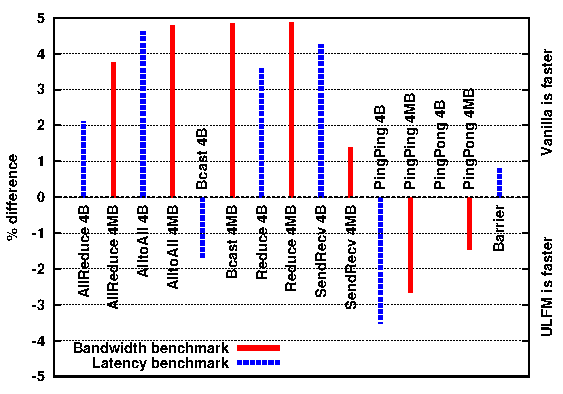
\includegraphics[width=\linewidth]{figures/IMB.pdf}\vspace{-.4cm}
 	\caption{IMB: \ulfm vs. Vanilla Open MPI (Romulus)
 	\label{fig:IMB}}
  \end{minipage}\vspace{-.3cm}
  \hfill
  \begin{minipage}[t]{0.48\linewidth}
    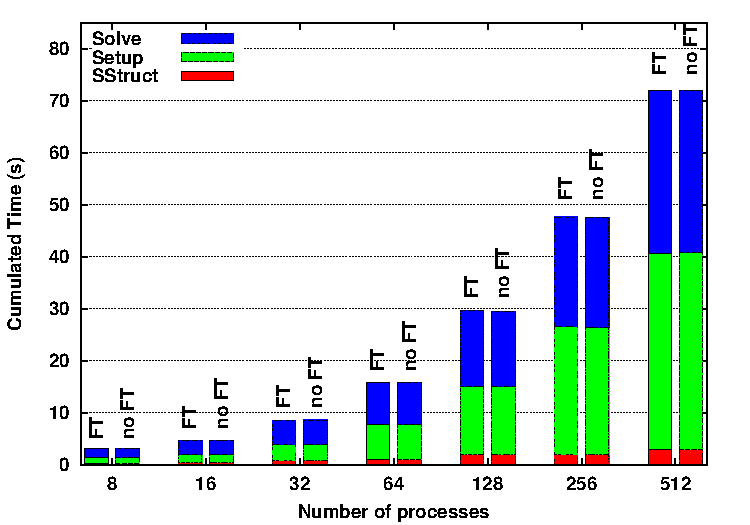
\includegraphics[width=\linewidth]{figures/bargraph.pdf}\vspace{-.4cm}
    \caption{Sequoia-AMG: \ulfm vs. Vanilla Open MPI at various scales (Smoky)
    \label{fig:sequoia:bargraph}}
  \end{minipage}\vspace{-.3cm}
\end{figure}

The impact on shared memory systems, sensitive to small modifications of
the MPI library, has been assessed on Romulus -- a large shared memory 
machine -- using the IMB benchmark suite (v3.2.3) as shown in 
Figure~\ref{fig:IMB}. The duration of all benchmarks remains below 5\%, 
within the standard deviation of the machine's implementation

To measure the impact of the prototype on a real application, we used the
Sequoia AMG benchmark\footnote{https://asc.llnl.gov/sequoia/benchmarks/\#amg}, 
an Algebraic Mult-Grid (AMG) linear system
solver for unstructured mesh physics. A weak scaling study was conducted up to
512 processes following the problem \emph{Set 5}.
Figure~\ref{fig:sequoia:bargraph} compares the time slicing of three main
phases (Solve, Setup, and SStruct) of the benchmark, with the
vanilla implementation of Open MPI, and the \ulfm enabled one. The
application itself is not fault tolerant and does not use the features proposed
in \ulfm. This benchmark demonstrates that a careful
implementation of \ulfm need not impact the performance of the
MPI implementation.
